\documentclass[12pt,a4paper,notitlepage]{report}
\usepackage[utf8]{inputenc}
\usepackage[english]{babel}

% AMS packages
\usepackage{amsmath}
\usepackage{amsfonts}
\usepackage{amssymb}

\usepackage{eurosym}% euros
\usepackage{listings} % code
% Images
\usepackage{graphicx}
\graphicspath{{images/}}
\usepackage[outdir=images/]{epstopdf}
\usepackage{subfigure}
\DeclareGraphicsExtensions{.pdf,.jpeg,.png,.eps}

\usepackage{todonotes}
\title{LINMA 2470 : Stochastic models}
\author{Quentin Laurent}
\begin{document}
\maketitle
\section*{Model}
We are going to model our bank as a $M/G/2$ queue. Hence the arrival times will follow an exponential law, and the distribution of service time is any distribution where times are positive.
\todo[inline]{Comment traiter le fait qu'un teller est parfois inactif?}
\section*{Parameters estimation}
In order to determine the arrival rate $\lambda (hr^{-1})$ of the clients in the bank we need to analyse the provided data.\\
If we assume that the number of people in the line at the end of the half-day is zero, then the number of people who arrived is equal to the number of people who were served by either one of the two tellers.\\
A more sophisticated approach would include time-varying arrival rate.
\todo[inline]{Traiter les données et montrer pourquoi c'est le meilleur estimateur}


\section*{Anylogic model}

\todo[inline]{Modèle anylogic}

\section*{The merge project}
 Since the clients arriving in the two old branches will sum up and go to the merged branch, we simply add the two Poisson processes, which gives us a new Poisson process with an arrival rate of the clients twice as big as that of the two old branches.

The question that now arises is how many tellers do we really need? Since in each bank a teller is idle at some time, how many of them are needed to make sure that the clients don't wait too much.


In order to estimate the number of tellers necessary for the merged bank, we perform a quasi-steady state approximation of the system. \todo[inline]{explain quasi-steady state approx}

We suppose that the number of tellers is constant throughout the half day considered.
We are trying to minimize a weighted function of the capacity and the total waiting time of the clients.
We consider that the cost of the capacity is proportional to $ \alpha$ (\euro s/customers), and the value of the waiting time of the clients is proportional to $\beta$ (\euro/$s^2$).

Hence, we simply solve the following program :

\begin{eqnarray*}
\min_c & & \alpha c + \beta \int_D A(t)-S(t)\\
\end{eqnarray*}
where $D = \{t | A(t)>=S(t) \}$

So let's now estimate the parameters. Let's say that we pay a teller $S = 75$\euro a day, taxes included.
The average processing time is denoted by $\mu$. 
The parameter $\alpha$ is given by $\alpha = \frac{S}{\mu}$
If we say that the time of a customer is worth as much as the time of our employee, then we would have $\beta = \frac{S}{tt}$ where $tt$ is the total number of seconds in a half day.\\
An example of parameters is given in table \ref{table:param}.
\begin{table}
\begin{tabular}{|c|c|c|c|}
\hline 
1/2 day salary(\euro ) & Half day time(s) & $\alpha$(\euro $s$/clients) & $\beta$(\euro/clients$\cdot s$) \\ 
 \hline 
$75$ & $10800$ & $0.433526$ & $3.47222e-07$ \\ 
 \hline 
 
 \end{tabular}
\caption{Parameters\label{table:param}}
\end{table}

Our optimisation problem gives us a value of $ 0.00805561 $ for $c$, which optimizes the capacity in customers per second.\\
It gives us the optimal number of tellers : $N_t = c \mu$
We can see on figure \ref{fig:clients_lun} the evolution of the clients arrived and the clients served during the afternoon of monday. We can see that at some point the serving rate of the clients cannot follow the arrival rate of the clients. From this point a queue starts growing until the arrival rate lowers and the queue is nearly empty again.
\begin{figure}[h]
\centering
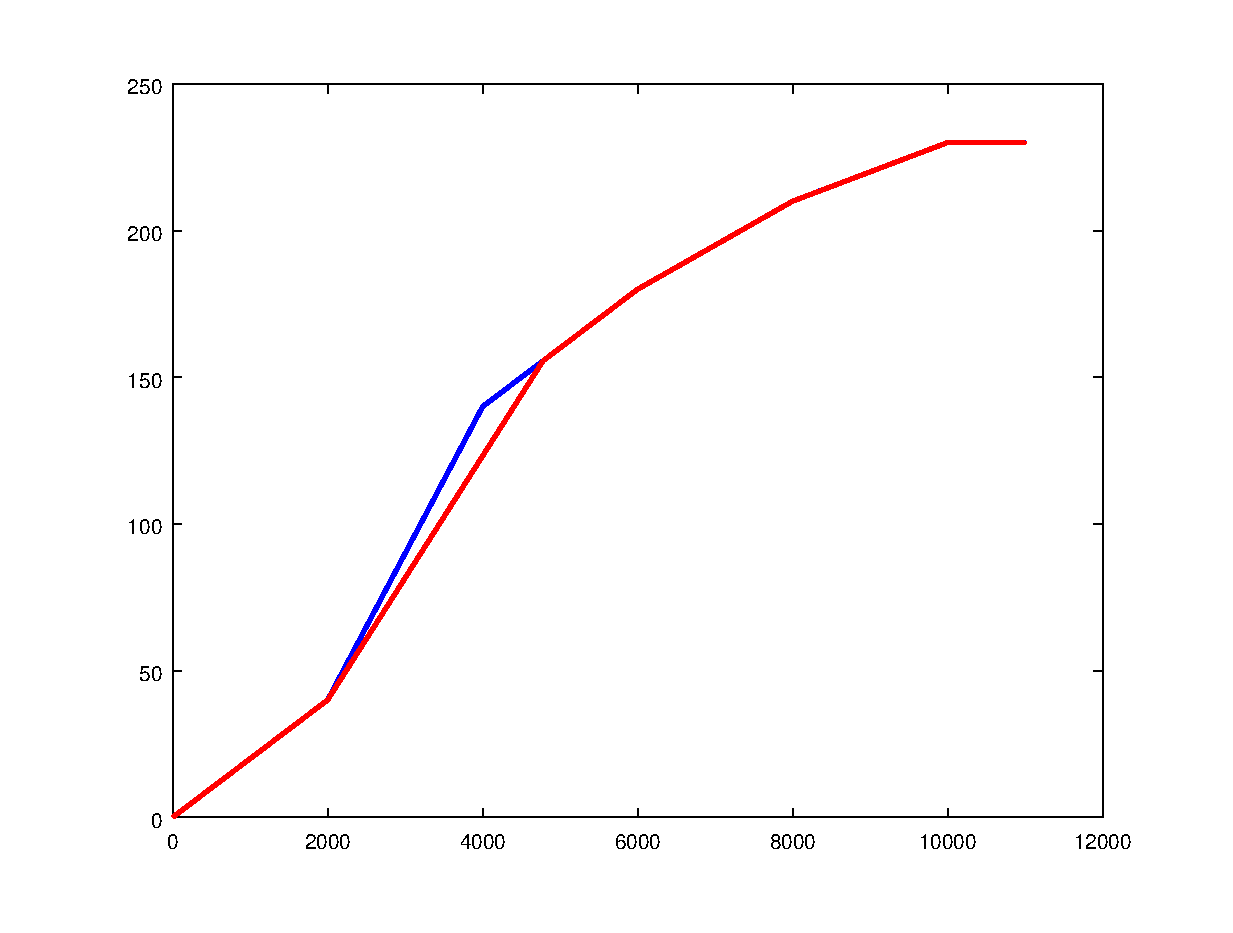
\includegraphics[width = 8cm]{half_day_test_clients_served.eps}
\caption{Cumulative amount of clients arrived and served\label{fig:clients_lun}}
\end{figure}

\end{document}